\section{Econometrics: Time-varying Bayesian VAR}
\label{chapter3_section6}

In a context of rapidly changing economic dynamics, static VAR models can be incapable of capturing the fast evolutions of the unerlying process and hence produce suboptimal forecasts. For this reason, a natural extention to VAR models consists in integrating dynamics in the model parameter themselves. The major contributions in the field are the papers by \cite{Primiceri2005} and \cite{DelNegro2015}. The presentation in this section follows the equation-by-equation approach proposed by \cite{Legrand2019}, which improves on both the calculation speed and prediction accuracy.

\subsection{Formulation}
\label{chapter3_section6_subsection1}

A general time-varying VAR model can be written as:

\begin{equation}
y_t = c_t + A_{1,t} y_{t-1} + \cdots + A_{p,t} y_{t-p} + \varepsilon_t \hspace{2cm}
\varepsilon_t \sim N(0, \Sigma_t)
\label{equation_c3_s6_ss1_1}
\end{equation}

This model is similar to \ref{equation_c3_s5_ss1_1}, except that the parameters $c_t, A_{1,t}, \cdots, A_{p,t}$ and $\Sigma_t$ are not allowed to be period-specific. Stacking in a vector $\beta_t$ the set of VAR coefficients, \ref{equation_c3_s6_ss1_1} rewrites:

\begin{equation}
y_t=X_t \beta_t+\varepsilon_t
\label{equation_c3_s6_ss1_2} 
\end{equation}

with:

\begin{equation}
X_t=I_n \otimes x_t \hspace{2mm} , \hspace{2mm} x_t=\left( \begin{matrix} z_t' & y_{t-1}' & \cdots & y_{t-p}' \\ \end{matrix} \right) \hspace{2mm} , \hspace{2mm} \beta_t=vec(B_t) \hspace{2mm} , \hspace{2mm} B_t=\left( \begin{matrix} C_t & A_{1,t} & \cdots & A_{p,t} \\ \end{matrix} \right)'
\label{equation_c3_s6_ss1_3}
\end{equation}


Considering specifically row $i$ of \ref{equation_c3_s6_ss1_2} , the equation for variable $i$ of the model rewrites:

\begin{equation}
y_{i,t}=x_t \beta_{i,t}+\varepsilon_{i,t}
\label{equation_c3_s6_ss1_4}
\end{equation}

where $\beta_{i,t}$ is the $k \times 1$ vector obtained from column $i$ of $B_t$. Stacking \ref{equation_c3_s6_ss1_4} over the $T$ sample periods yields a full sample formulation for equation $i$:

\begin{equation}
y_i= X \beta_i+\varepsilon_i
\label{equation_c3_s6_ss1_5} 
\end{equation}

with:

\begin{equation}
y_i=\left( \begin{matrix} y_{i,1} \\ y_{i,2} \\ \vdots \\ y_{i,T} \\ \end{matrix} \right)
\hspace{4mm} , \hspace{4mm}
X=\left( \begin{matrix} x_1 & 0 & \cdots & 0 \\ 0 & x_2 & \ddots & \vdots \\ \vdots & \ddots & \ddots & 0 \\ 0 & \cdots & 0 & x_T \\ \end{matrix} \right)
\hspace{4mm} , \hspace{4mm}
\beta_i=\left( \begin{matrix} \beta_{i,1} \\ \beta_{i,2} \\ \vdots \\ \beta_{i,T} \\ \end{matrix} \right)
\hspace{4mm} , \hspace{4mm}
\varepsilon_i=\left( \begin{matrix} \varepsilon_{i,1} \\ \varepsilon_{i,2} \\ \vdots \\ \varepsilon_{i,T} \\ \end{matrix} \right)
\label{equation_c3_s6_ss1_6} 
\end{equation}

The variance-covariance matrix $\Sigma_t$ for the reduced form residuals is decomposed into:

\begin{equation}
\Delta_t \Sigma_t \Delta_t'=\Lambda_t \hspace{10mm} \Leftrightarrow \hspace{10mm} \Sigma_t=\Delta_t^{-1} \Lambda_t \Delta_t^{-1}\phantom{}'
\label{equation_c3_s6_ss1_7} 
\end{equation}

$\Delta_t$ (and $\Delta_t^{-1}$) are unit lower triangular matrix, while $\Lambda_t$ is a diagonal matrix with positive diagonal entries, taking the form:

\begin{equation}
\Delta_t=\left( \begin{matrix} 1 & 0 & \cdots & 0 \\ \delta_{21,t} & 1 & \ddots & \vdots \\ \vdots & \ddots & \ddots & 0 \\ \delta_{n1,t} & \cdots & \delta_{n(n-1),t} & 1 \end{matrix} \right)
\hspace{1mm} , \hspace{1mm}
\Lambda_t=\left( \begin{matrix} s_1 \ exp(\lambda_{1,t}) & 0 & \cdots & 0 \\ 0 & s_2 \ exp(\lambda_{2,t}) & \ddots & \vdots \\ \vdots & \ddots & \ddots & 0 \\ 0 & \cdots & 0 & s_n \ exp(\lambda_{n,t}) \\ \end{matrix} \right)
\label{equation_c3_s6_ss1_8} 
\end{equation}

The triangular decomposition of the variance-covariance matrix $\Sigma_t$ implemented in \ref{equation_c3_s6_ss1_7} is common in time-series models. $\Lambda_t$ represents the volatility components of $\Sigma_t$, each $s_i$ being a positive scaling term which represents the equilibrium value of the residual variance of equation $i$ of the model. On the other hand, $\Delta_t$ can be interpreted as the (inverse) covariance component of $\Sigma_t$. Denoting by $\delta_{i,t}$ the vector of non-zero and non-one terms in row $i$ of $\Delta_t$ so that $\delta_{i,t} = ( \begin{matrix} \delta_{i1,t} & \cdots & \delta_{i(i-1),t} \end{matrix} )'$, $\delta_{i,t}$ then represents the covariance between the residual of equation $i$ of the model and the other shocks.

The dynamics of the model time-varying parameters is specified as follows:

\begin{lflalign}
\beta_{i,t}=(1-\rho_i) b_i+ \rho_i \beta_{i,t-1} +\xi_{i,t} \hspace{19.5mm} t=2,3,\ldots,T \hspace{15mm} \xi_{i,t} \sim \No(0,\Omega_i) \nonumber \\
\beta_{i,1}=b_i +\xi_{i,1} \hspace{49mm} t=1 \hspace{30mm} \xi_{i,1} \sim \No \left( 0,\tau \Omega_i \right) \nonumber \\
\lambda_{i,t}= \gamma_i \lambda_{i,t-1} +\nu_{i,t} \hspace{40mm} t=2,3,\ldots,T \hspace{15mm} \nu_{i,t} \sim \No(0,\phi_i) \nonumber \\
\lambda_{i,1}=\nu_{i,1}  \hspace{56.5mm} t=1 \hspace{30mm} \nu_{i,1} \sim \No \left( 0,\mu \phi_i \right)  \nonumber \\
\delta_{i,t}= (1-\alpha_i) d_i + \alpha_i \delta_{i,t-1} + \eta_{i,t} \hspace{19mm} t=2,3,\ldots,T \hspace{15mm} \eta_{i,t} \sim \No(0,\Psi_i) \nonumber \\
\delta_{i,1}= d_i + \eta_{i,1} \hspace{49mm} t=1 \hspace{30mm} \eta_{i,1} \sim \No(0, \eps \Psi_i)
\label{equation_c3_s6_ss1_9} 
\end{lflalign}

$\rho_i$, $\gamma_i$ and $\alpha_i$ represent equation-specific autoregressive coefficients while $b_i$, $s_i$ and $d_i$ represent the equation-specific mean values of the processes. These values are exogenous hyperparameters sepcified by the user. For each process, the initial period is formulated consistently with the overall dynamics of the parameters. The mean corresponds to the unconditional expectation of the process, while the variance is scaled by the hyperparameters $\tau, \mu, \eps \ > 1$ to account for the greater uncertainty associated with the initial period. All the innovations in the model are assumed to be jointly normally distributed with the following assumptions on the variance covariance matrix:

\begin{equation}
Var \left( \begin{matrix} \varepsilon_t \\ \xi_{i,t} \\ \nu_{i,t} \\ \eta_{i,t} \end{matrix} \right) = \left( \begin{matrix} \Sigma_t & 0 & 0 & 0 \\ 0 & \Omega_i & 0 & 0 \\ 0 & 0 & \phi_i & 0 \\ 0 & 0 & 0 & \Psi_i \end{matrix} \right)
\label{equation_c3_s6_ss1_10} 
\end{equation}



\subsection{Estimation}
\label{chapter3_section6_subsection2}


For $i=1, \ldots, n$, the parameters of interest to be estimated are: the dynamic VAR coefficients $\beta_i$ ; the dynamic volatility terms $\lambda_i$; the dynamic covariance terms $\delta_i$; and the associated variance-covariance parameters $\Omega_i$, $\phi_i$ and $\Psi_i$. To these six base parameters must be added the parameter $r_{i,t}$ whose role will be clarified shortly.
Given the model, Bayes rule is given by: 

\begin{lflalign}
\ & \ \pi( \beta, \Omega, \lambda, \phi, \delta, \Psi, r|y) \propto f(y|\beta, \lambda, \delta, r) \nonumber \\
\times \ & \ \left( \prod \limits_{i=1}^{n}{\pi(\beta_i|\Omega_i) \pi(\Omega_i) } \right) \left( \prod \limits_{i=1}^{n}{\pi(\lambda_i|\phi_i) \pi(\phi_i)} \right) \left( \prod \limits_{i=2}^{n}{\pi(\delta_i|\Psi_i) \pi(\Psi_i)} \right) \left( \prod \limits_{i=1}^{n}{\prod \limits_{t=1}^{T}{\pi(r_{i,t})}} \right)
\label{equation_c3_s6_ss2_1} 
\end{lflalign}

\newpage

From \ref{equation_c3_s6_ss1_2}, an immediate formulation of the likelihood function obtains as:

\begin{equation}
f(y| \beta, \lambda, \delta, r) = \prod \limits_{t=1}^{T}{(2\pi )^{-n/2} |\Sigma_t|^{-1/2} exp \left(-\frac{1}{2} (y_t-X_t \beta_t)' \Sigma_t^{-1} (y_t-X_t \beta_t) \right)}
\label{equation_c3_s6_ss2_2}
\end{equation}

The priors for $\beta_i, \lambda_i$ and $\delta_i$ are fully defined by their dynamic equations in \ref{equation_c3_s6_ss1_9}.

The prior distributions for the variance parameters $\Omega_i, \phi_i$ and $\Psi_i$ are standard inverse Wishart and inverse Gamma distributions. For $\Omega_i$, the prior is inverse Wishart with degrees of freedom $\zeta_0$ and scale $\Upsilon_0$:

\begin{equation}
\pi(\Omega_i) \sim IW \left( \zeta_0,\Upsilon_0 \right)
\label{equation_c3_s6_ss2_3} 
\end{equation}

Following:

\begin{equation}
\pi(\Omega_i)=\frac{2^{-\zeta_0 k/2}}{\Gamma_k \left( \frac{\zeta_0}{2} \right)} |\Upsilon_0|^{\zeta_0/2} |\Omega_i|^{-(\zeta_0+k+1)/2} exp \left( -\frac{1}{2} tr \left\{ \Omega_i^{-1} \Upsilon_0 \right\} \right)
\label{equation_c3_s6_ss2_4} 
\end{equation}

The prior distribution for each $\phi_i$ is inverse gamma with shape $\frac{\kappa_0}{2}$ and scale $\frac{\omega_0}{2}$:

\begin{equation}
\pi(\phi_i) \sim IG \left( \frac{\kappa_0}{2},\frac{\omega_0}{2} \right)
\label{equation_c3_s6_ss2_5}
\end{equation}

Hence:

\begin{equation}
\pi(\phi_i)=\frac{\frac{\omega_0}{2}^{\kappa_0/2}}{\Gamma(\frac{\kappa_0}{2})} \phi_i^{-\kappa_0/2-1} exp \left( - \frac{\omega_0}{2\phi_i} \right)
\label{equation_c3_s6_ss2_6}
\end{equation}

Finally, the prior distribution for $\Psi_i$ is inverse Wishart with degrees of freedom $\varphi_0$ and scale $\Theta_0$:

\begin{equation}
\pi(\Psi_i) \sim IW \left( \varphi_0,\Theta_0 \right)
\label{equation_c3_s6_ss2_7} 
\end{equation}

Following:

\begin{equation}
\pi(\Psi_i)=\frac{2^{-\varphi_0 (i-1)/2}}{\Gamma_{(i-1)} \left( \frac{\varphi_0}{2} \right)} |\Theta_0|^{\varphi_0/2} |\Psi_i|^{-(\varphi_0+(i-1)+1)/2} exp \left( -\frac{1}{2} tr \left\{ \Psi_i^{-1} \Theta_0 \right\} \right)
\label{equation_c3_s6_ss2_8}
\end{equation}

\newpage

Bayes rule \ref{equation_c3_s6_ss2_1} is intractable, and requires the use of MCMC methods. As usual, the Gibbs sampling algorithm is used, relying on the conditional posterior. From Bayes rule \ref{equation_c3_s6_ss2_1}, one obtains that the conditional posterior $\pi(\beta_i | y, \backslash \beta_i)$ is given by $\pi(\beta_i | y, \backslash \beta_i) \propto f(y | \beta, \lambda, \delta, r) \pi(\beta_i | \Omega_i)$. Starting from \ref{equation_c3_s6_ss2_2}, and after some manipulations, the likelihood function $f(y | \beta, \lambda, \delta, r)$ reformulates as:

\begin{equation}
y_{i,t}+\delta_{i,t}' \varepsilon_{-i,t}=x_t \beta_{i,t}+ e_{i,t} \hspace{10mm} e_{i,t} \sim \No(0,s_i \ exp(\lambda_{i,t}))
\label{equation_c3_s6_ss2_9} 
\end{equation}

where $\varepsilon_{-i,t} = (\varepsilon_{1,t} \cdots \varepsilon_{i-1,t})$. \ref{equation_c3_s6_ss2_9} and \ref{equation_c3_s6_ss1_9} respectively provide the observation and state equations for the dynamic parameter $\beta_i$. The conditional posterior $\pi(\beta_i | y, \backslash \beta_i)$ can then be recovered from the Carter-Kohn algorithm (see Appendix \ref{appendix3} for the details of the algorithm).

From Bayes rule \ref{equation_c3_s6_ss2_1}, one obtains that the conditional posterior $\pi(\delta_i | y, \backslash \delta_i)$ is given by $\pi(\delta_i | y, \backslash \delta_i) \propto f(y | \beta, \lambda, \delta, r) \pi(\delta_i | \Psi_i)$. Starting from \ref{equation_c3_s6_ss2_2}, and after some manipulations, the likelihood function $f(y | \beta, \lambda, \delta, r)$ reformulates as:

\begin{equation}
\varepsilon_{i,t}=-\varepsilon_{-i,t}' \delta_{i,t}+ e_{i,t} \hspace{10mm} e_{i,t} \sim \No (0,s_i \ exp(\lambda_{i,t}))
\label{equation_c3_s6_ss2_10}
\end{equation}

\ref{equation_c3_s6_ss2_10} and \ref{equation_c3_s6_ss1_9} respectively provide the observation and state equations for the dynamic parameter $\delta_i$. The conditional posterior $\pi(\delta_i | y, \backslash \delta_i)$ can then be recovered from the Carter-Kohn algorithm.

From Bayes rule \ref{equation_c3_s6_ss2_1}, one obtains that the conditional posterior $\pi(\lambda_i | y, \backslash \lambda_i)$ is given by $\pi(\lambda_i | y, \backslash \lambda_i) \propto f(y | \beta, \lambda, \delta, r) \pi(\lambda_i | \phi_i)$. As it is, the likelihood function \ref{equation_c3_s6_ss2_2} is not workable due to the exponential terms in \ref{equation_c3_s6_ss1_8}. \cite{Kim1998} thus propose to approximate the likelihood with a mixture of 7 normal distributions, where the mixture component is determined by the categorical random variable $r_{i,t}$ taking value $j= 1, 2, \cdots, 7$. The likelihood function then rewrites as:

\begin{equation}
\hat{y}_{i,t} - m_j = \lambda_{i,t} + \hat{e}_{i,t} \hspace{10mm} \hat{e}_{i,t} \sim \No (0,v_j)
\label{equation_c3_s6_ss2_11} 
\end{equation}

where $\hat{y}_{i,t} = \log(s_i^{-1} [\varepsilon_{i,t} + \varepsilon_{-i,t}' \delta_{i,t}])$ and $m_j$ and $v_j$ denote the respective mean and variance of the normal distribution when the random variable $r_{i,t}$ selects the mixture component $j$. \ref{equation_c3_s6_ss2_11} and \ref{equation_c3_s6_ss1_9} respectively provide the observation and state equations for the dynamic parameter $\delta_i$. The conditional posterior $\pi(\delta_i | y, \backslash \delta_i)$ can then be recovered from the Carter-Kohn algorithm.

From Bayes rule \ref{equation_c3_s6_ss2_1}, one obtains that the conditional posterior $\pi(r_{i,t}|y, \backslash r_{i,t})$ is given by $\pi(r_{i,t}|y, \backslash r_{i,t}) \propto f(y|\beta, \lambda, \delta, r) \pi(r_{i,t})$. Given that $r_{i,t}$ is a categorical random variable, and some rearrangements of the approximated $f(y|\beta, \lambda, \delta, r)$, one eventually obtains:

\begin{equation}
\pi(r_{i,t}|y, \backslash r_{i,t}) \propto \bar{q}_j^{\hspace{0.5mm} \ind(r_{i,t}=j)}
\label{equation_c3_s6_ss2_12} 
\end{equation}

with:

\begin{equation}
\bar{q}_j=(2\pi v_j)^{-1/2} \exp\left(-\frac{1}{2} \frac{(\hat{y}_{i,t}-\lambda_{i,t}-m_j)^2}{v_j} \right) q_j
\label{equation_c3_s6_ss2_13} 
\end{equation}

This is the kernel of a categorical distribution with probabilities $\bar{q}_1,\bar{q}_2,\ldots,\bar{q}_7$:
 $\pi(r_{i,t}|y, \backslash r_{i,t}) \sim Cat(\bar{q}_1,\bar{q}_2,\ldots,\bar{q}_7)$.

The conditional posteriors for the variance terms are standard. For $\Omega_i$, start from Bayes rule \ref{equation_c3_s6_ss2_1} and relegate to the normalising constant any multiplicative term not involving $\Omega_i$ to obtain:

\begin{equation}
\pi(\Omega_i |y, \backslash \Omega_i) \propto \pi(\beta_i|\Omega_i) \pi(\Omega_i)
\label{equation_c3_s6_ss2_14} 
\end{equation}

Given the priors \ref{equation_c3_s6_ss1_9}  and \ref{equation_c3_s6_ss2_4} and rearranging yields:

\begin{equation}
\pi(\Omega_i |y, \backslash \Omega_i) = |\Omega_i|^{-(\bar{\zeta}+k+1)/2} exp \left( -\frac{1}{2} tr \left\{ \Omega_i^{-1} \bar{\Upsilon}_i \right\} \right)
\label{equation_c3_s6_ss2_15}
\end{equation}

with:

\begin{lflalign}
\bar{\zeta}=T+\zeta_0 \qquad \bar{\Upsilon}_i=\tilde{B}_i + \Upsilon_0 \nonumber \\
\tilde{B}_i=(B_i-1_T' \otimes b_i) \ (F_i' \ I_{-\tau} \ F_i) (B_i-1_T' \otimes b_i)' \qquad B_i=\left( \begin{matrix} \beta_{i,1} & \beta_{i,2} & \cdots & \beta_{i,T} \end{matrix} \right) \nonumber \\
F_i=\left( \begin{matrix} 1 & 0 & \cdots & 0 \\ -\rho_i & 1 & \ddots & \vdots \\ \vdots & \ddots & \ddots & 0 \\ 0 & \cdots & -\rho_i & 1 \\ \end{matrix} \right) \qquad I_{-\tau} = \left( \begin{matrix} \tau^{-1} & 0 & \cdots & 0 \\ 0 & 1 & \ddots & \vdots \\ \vdots & \ddots & \ddots & 0 \\ 0 & \cdots & 0 & 1 \end{matrix} \right)
\label{equation_c3_s6_ss2_16}
\end{lflalign}

This is the kernel of an inverse Wishart distribution with degrees of freedom $\bar{\zeta}$ and scale $\bar{\Upsilon}_i$: $\pi(\Omega_i |y, \backslash \Omega_i) \sim IW (\bar{\zeta},\bar{\Upsilon}_i)$

\newpage

For $\phi_i$, start from Bayes rule \ref{equation_c3_s6_ss2_1} and relegate to the normalising constant any multiplicative term not involving $\phi_i$ to obtain:

\begin{equation}
\pi(\phi_i |y, \backslash \phi_i) \propto \pi(\lambda_i|\phi_i) \pi(\phi_i)
\label{equation_c3_s6_ss2_17} 
\end{equation}

Given the priors \ref{equation_c3_s6_ss1_9}  and \ref{equation_c3_s6_ss2_6} and rearranging yields:

\begin{equation}
\pi(\phi_i |y, \backslash \phi_i) \propto \phi_i^{-\bar{\kappa}-1} exp \left( - \frac{\bar{\omega}_i}{\phi_i} \right)
\label{equation_c3_s6_ss2_18}  
\end{equation}

with: 

\begin{lflalign}
\bar{\kappa}=\frac{T+\kappa_0}{2}
 \qquad \bar{\omega}_i=\frac{\lambda_i'  (G_i' I_{-\mu} G_i) \lambda_i+\omega_0}{2} \nonumber \\
G_i = \left( \begin{matrix} 1 & 0 & \cdots & 0 \\ -\gamma_i & 1 & \ddots & \vdots \\ \vdots & \ddots & \ddots & 0 \\ 0 & \cdots & -\gamma_i & 1 \\ \end{matrix} \right) \qquad I_{-\mu} = \left( \begin{matrix} \mu^{-1} & 0 & \cdots & 0 \\ 0 & 1 & \ddots & \vdots \\ \vdots & \ddots & \ddots & 0 \\ 0 & \cdots & 0 & 1 \end{matrix} \right)
\label{equation_c3_s6_ss2_19} 
\end{lflalign}

This is the kernel of an inverse Gamma distribution with shape $\bar{\kappa}$ and scale $\bar{\omega}_i$: $\pi(\phi_i |y, \backslash \phi_i) \sim IG (\bar{\kappa}, \bar{\omega}_i)$

Finally, for $\Psi_i$, start from Bayes rule \ref{equation_c3_s6_ss2_1} and relegate to the normalising constant any multiplicative term not involving $\Psi_i$ to obtain:

\begin{equation}
\pi(\Psi_i |y, \backslash \Psi_i) \propto \pi(\delta_i|\Psi_i) \pi(\Psi_i)
\label{equation_c3_s6_ss2_20}  
\end{equation}

Given the priors \ref{equation_c3_s6_ss1_9}  and \ref{equation_c3_s6_ss2_8} and rearranging yields:

\begin{equation}
\pi(\Psi_i |y, \backslash \Psi_i) \propto |\Psi_i|^{-(\bar{\varphi}+(i-1)+1)/2} exp \left( -\frac{1}{2} tr \left\{ \Psi_i^{-1} \bar{\Theta}_i \right\} \right)
\label{equation_c3_s6_ss2_21}
\end{equation}

with: 

\begin{lflalign}
\bar{\varphi}=T+\varphi_0
 \qquad \bar{\Theta}_i=\tilde{D}_i+\Theta_0 \nonumber \\
\tilde{D}_i= (D_i-1_T' \otimes d_i) \ (H_i' \ I_{-\eps} \ H_i) (D_i-1_T' \otimes d_i)' \qquad  D_i= \left( \begin{matrix} \delta_{i,1} & \delta_{i,2} & \cdots & \delta_{i,T} \end{matrix} \right) \nonumber \\
H_i= \left( \begin{matrix} 1 & 0 & \cdots & 0 \\ -\alpha_i & 1 & \ddots & \vdots \\ \vdots & \ddots & \ddots & 0 \\ 0 & \cdots & -\alpha_i & 1 \\ \end{matrix} \right) \qquad I_{-\eps} = \left( \begin{matrix} \eps^{-1} & 0 & \cdots & 0 \\ 0 & 1 & \ddots & \vdots \\ \vdots & \ddots & \ddots & 0 \\ 0 & \cdots & 0 & 1 \\ \end{matrix} \right)
\label{equation_c3_s6_ss2_22} 
\end{lflalign}

This is the kernel of an inverse Wishart distribution with degrees of freedom $\bar{\varphi}$ and scale $ \bar{\Theta}_i$: $\pi(\Psi_i |y, \backslash \Psi_i) \sim IW (\bar{\varphi}, \bar{\Theta}_i)$

It is then possible to describe the full Gibbs sampling algorithm for the time-varying Bayesian VAR model:

\textbf{Algorithm 7: Gibbs sampling for the time-varying Bayesian VAR} \vspace{3mm} \\
1. Initiate $\beta_i^{(0)}, \lambda_i^{(0)}, \delta_i^{(0)}, \Omega_i^{(0)}, \phi_i^{(0)}, \delta_i^{(0)}$ and $r_{i,t}^{(0)}$ with any values, for $i=1,\cdots,n$ and $t=1,\cdots,T$. In practice, use static OLS estimates for each variable and each period. Also decide the total number of repetitions of the algorithm (say $r$=2000 for instance), and the number of initial iterations to discard (for instance $d$ = 1000) to ensure convergence.

2. For $i=1, \ldots, n$, sample $\lambda_i^{(n)}$ equation by equation, using the Carter-Kohn algorithm.

3. For $i=1, \ldots, n$, sample $\beta_i^{(n)}$ equation by equation, using the Carter-Kohn algorithm.

4. For $i=2, \ldots, n$, sample  $\delta_i^{(n)}$ equation by equation, using the Carter-Kohn algorithm.

5. For $i=1, \ldots, n$, sample $\Omega_i^{(n)}$ equation by equation from: $\pi(\Omega_i^{(n)} |y, \backslash \Omega_i) \sim IW (\bar{\zeta},\bar{\Upsilon}_i)$.

6. For $i=1, \ldots, n$, sample $\phi_i^{(n)}$ equation by equation from: $\pi(\phi_i^{(n)} |y, \backslash \phi_i) \sim IG(\bar{\kappa},\bar{\omega}_i)$.

7. For $i=2, \ldots, n$, sample $\Psi_i^{(n)}$ equation by equation from: $\pi(\Psi_i^{(n)} |y, \backslash \Psi_i) \sim IW (\bar{\varphi},\bar{\Theta}_i)$.

8. For $i=1, \ldots, n$ and $t=1,\ldots,T$, sample $r_{i,t}^{(n)}$ from: $\pi(r_{i,t}^{(n)}|y, \backslash r_{i,t}) \sim Cat(\bar{q}_1,\ldots,\bar{q}_7)$.

9. Repeat $r$ times.

10. Discard $d$ initial observations as burn-in sample to make sure convergence is achieved. Then the remaining values are draws from the unconditional posteriors $\pi(\beta| y)$ and $\pi(\Sigma| y)$, which can be used to recover an empirical distribution.

\newpage

\subsection{Prediction}
\label{chapter3_section6_subsection3}


The MCMC algorithm for predictions is given by:

\textbf{Algorithm 8: prediction for the time-varying Bayesian VAR} \vspace{3mm} \\
1. for $i=1,\cdots, n$, draw values for $\lambda_i, \delta_i, \phi_i$ and $\Psi_i$ from their conditional posteriors. Recycle draws from the Gibbs sampling algorithm.

2. for $i=1,\cdots, n$, obtain values for $\lambda_{i,t+1}, \delta_{i,t+1}, \cdots, \lambda_{i,t+h}, \delta_{i,t+h}$ from \ref{equation_c3_s6_ss1_9}. Recover $\Sigma_{t+1}, \cdots, \Sigma_{t+h}$ from \ref{equation_c3_s6_ss1_7} .

3. for $i=1,\cdots, n$, draw values for $\beta_i$ and $\Omega_i$ from their conditional posteriors. Recycle draws from the Gibbs sampling algorithm.

4. for $i=1,\cdots, n$, obtain values for $\beta_{i,t+1}, \cdots, \beta_{i,t+h}$ from \ref{equation_c3_s6_ss1_9}.

5. for $i=1,\cdots, n$, compute recursively $y_{i, t+1}, \cdots, y_{i, t+h}$ from \ref{equation_c3_s6_ss1_1}.

6. repeat the process $r-d$ times to obtain $r-d$ draws from the posterior predictive distribution.

\newpage

\subsection{Application}
\label{chapter3_section6_subsection4}


As an illustration, the estimates of the time-varying variances for the feature shocks are provided in Figure \ref{fig_c3_s6_ss4_1}. \vspace{-5mm}

\begin{figure}[H]
\centering
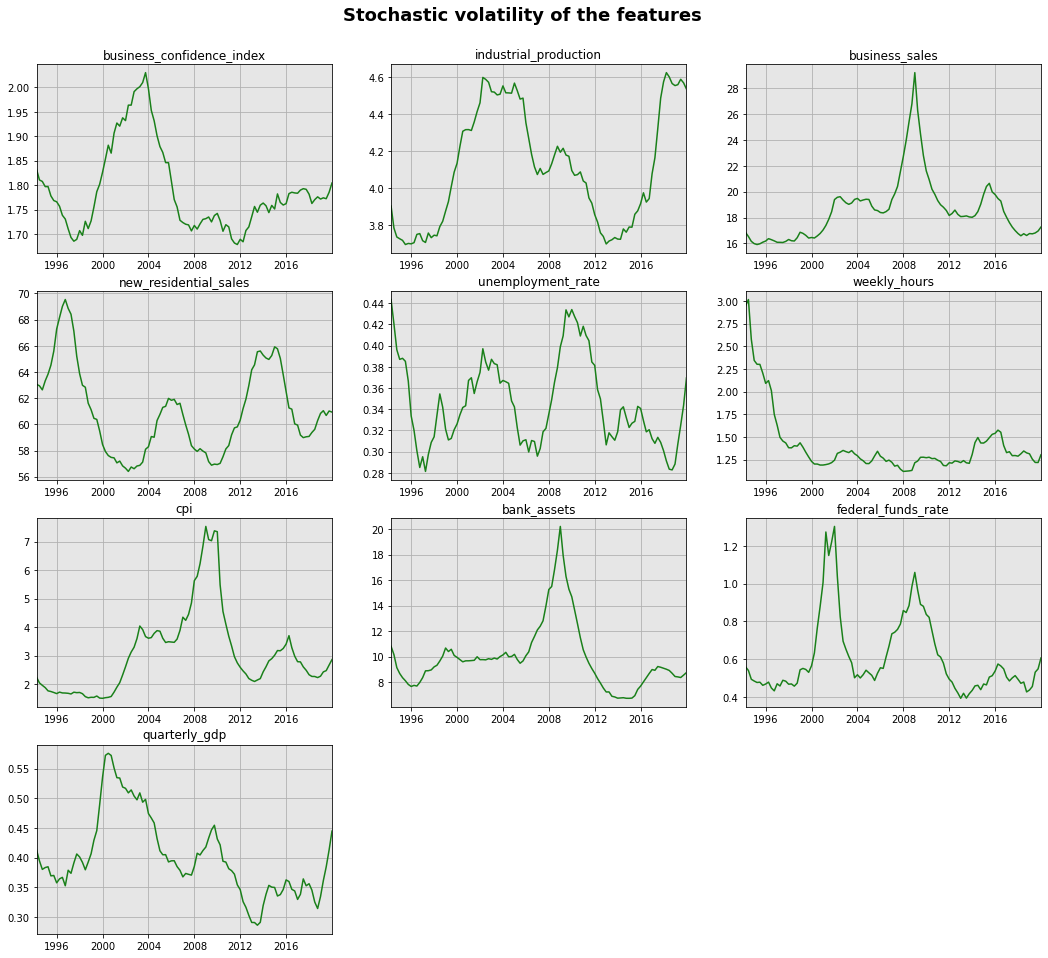
\includegraphics[scale=0.44]{images/stochastic_volatility.png}
\caption{Estimates of the time-varying feature variances}
\label{fig_c3_s6_ss4_1} \vspace{-5mm}
\end{figure}

The 2008 crisis is well pictured in many series, with a fueling in volatility (business sales, unemployment rate, bank assets, federal funds rate, quarterly GDP) over the period. Interestingly enough, the volatility in residential sales plumetted with the crisis, perhaps the sign that activity got stuck at a very low level over the period. Still worth noting, the model seems capable of anticipating the current crisis, with a rise in volatility of many key features over 2019, in particular industrial production, unemployment, the federal funds rate, and quarterly GDP.



\newpage
